\documentclass[10pt,winfonts,fancyhdr,hyperref,UTF8]{ctexrep}
\usepackage{indentfirst} 
\usepackage{fontspec}
\usepackage{titlesec}
\usepackage{xeCJK}
\usepackage{graphicx}
\usepackage{ifthen}
\usepackage{color,fancyvrb}
\usepackage{listings}
\usepackage{syntonly}
\usepackage{makeidx}
\usepackage[hidelinks, colorlinks=true]{hyperref}
\usepackage{algorithm}
\usepackage{algpseudocode}
\usepackage{amssymb}
\usepackage{multirow}
\usepackage{ulem}
\usepackage{diagbox}
\makeatletter
%LeetCode Setting
\usepackage[centering,paperwidth=180mm,paperheight=230mm,%
body={390pt,530pt},marginparsep=10pt,marginpar=50pt]{geometry}
\usepackage{color}
\usepackage{enumitem}
\usepackage{fancyvrb}
\usepackage[bottom,perpage,symbol*]{footmisc}
\usepackage{graphicx}
\usepackage[hidelinks]{hyperref}
\usepackage{makeidx}
\usepackage[toc]{multitoc}
\usepackage{pifont}
\usepackage{underscore}
\usepackage{amsmath}

\DefineFNsymbols*{chinese}{{\ding{172}}{\ding{173}}{\ding{174}}{\ding{175}}%
{\ding{176}}{\ding{177}}{\ding{178}}{\ding{179}}{\ding{180}}{\ding{181}}}
\setfnsymbol{chinese}

\hypersetup{bookmarksnumbered=true,bookmarksdepth=2}

\CTEXsetup[number={\thechapter}]{chapter}
\CTEXsetup[format+={\raggedleft}]{chapter}
\CTEXsetup[beforeskip={10pt}]{chapter}
\CTEXsetup[afterskip={30pt}]{chapter}
\def\CTEX@chapter@aftername{\par} % \CTEXsetup[aftername={\par}]{chapter}
\CTEXsetup[format+={\raggedright}]{section}
\CTEXsetup[beforeskip={-3.0ex plus -1ex minus -.2ex}]{section}
\CTEXsetup[afterskip={2.3ex plus .2ex minus 0.2ex}]{section}

\renewcommand \thefigure{\thechapter-\arabic{figure}}
\renewcommand \thetable{\thechapter-\arabic{table}}

\newcommand\figcaption[1]{\def\@captype{figure}\caption{#1}}
\newcommand\tabcaption[1]{\def\@captype{table}\caption{#1}}

\long\def\@caption#1[#2]#3{%
  \addcontentsline{\csname ext@#1\endcsname}{#1}%
    {\protect\numberline{\csname fnum@#1\endcsname}{ \ignorespaces #2}}% change "the" to "fnum@"
    \normalsize
    \@makecaption{\csname fnum@#1\endcsname}{\ignorespaces #3}}

\long\def\@makecaption#1#2{%
  \vskip\abovecaptionskip
  \sbox\@tempboxa{#1\quad#2}%
  \ifdim \wd\@tempboxa >\hsize
    #1\quad#2\par
  \else
    \global \@minipagefalse
    \hb@xt@\hsize{\hfil\box\@tempboxa\hfil}%
  \fi
  \vskip\belowcaptionskip}

\setlength\abovecaptionskip{0pt}
  
\setmainfont{Times New Roman}
%\setmainfont{Linux Libertine}
%\setmainfont{TeX Gyre Pagella}
\newfontfamily\urlfont{Times New Roman}
%\setmonofont[AutoFakeBold=1.6,AutoFakeSlant=0.17,Mapping=tex-text-tt]{Inconsolata}
\setCJKfamilyfont{zhyou}{YouYuan}

\newcommand{\fn}[1]{\texttt{#1}}
\newcommand{\sfn}[1]{\texttt{\small #1}}
\newcommand{\kw}[1]{\textsf{#1}}
\newcommand{\myurl}[1]{{\urlfont #1}}
\newcommand{\mpar}[1]{\marginpar[\hfill\kaishu #1]{\kaishu #1}}
\newcommand{\mn}[1]{\texttt{\bs #1}}
\renewcommand{\today}{\the\year-\the\month-\the\day}
\newcommand\bs{\textbackslash}
\newcommand{\code}[1]{\small{\fontspec{Latin Modern Mono} #1}}

\newcommand\begindot{\begin{itemize}
[itemsep=2pt plus 2pt minus 2pt,%
topsep=3pt plus 2pt minus 2pt,%
parsep=0pt plus 2pt minus 2pt]}
\newcommand\myenddot{\end{itemize}}

\newcommand\beginnum{\begin{enumerate}
[itemsep=2pt plus 2pt minus 2pt,%
topsep=3pt plus 2pt minus 2pt,%
parsep=0pt plus 2pt minus 2pt]}
\newcommand\myendnum{\end{enumerate}}

\DefineVerbatimEnvironment%
  {Code}{Verbatim}
  {fontsize=\small,baselinestretch=0.9,xleftmargin=3mm}

\raggedbottom
%\setlength{\parskip}{1ex plus .5ex minus .5ex}

\def\FV@SetLineWidth{%
  \if@FV@ResetMargins\else
    \advance\leftmargin\@totalleftmargin
  \fi
  \advance\leftmargin\FV@XLeftMargin\relax
  \advance\rightmargin\FV@XRightMargin\relax
  \linewidth\hsize
  %\advance\linewidth-\leftmargin
  %\advance\linewidth-\rightmargin
  \hfuzz\FancyVerbHFuzz\relax}


\def\FV@SingleFrameLine#1{%
%% DG/SR modification end
  \hbox to\z@{%
    %\kern\leftmargin
%% DG/SR modification begin - Jun. 22, 1998
    \ifnum#1=\z@
      \let\FV@Label\FV@LabelBegin
    \else
      \let\FV@Label\FV@LabelEnd
    \fi
    \ifx\FV@Label\relax
%% DG/SR modification end
      \FancyVerbRuleColor{\vrule \@width\linewidth \@height\FV@FrameRule}%
%% DG/SR modification begin - Jun. 22, 1998
    \else
      \ifnum#1=\z@
        \setbox\z@\hbox{\strut\enspace\urlfont\FV@LabelBegin\strut}%
      \else
        \setbox\z@\hbox{\strut\enspace\urlfont\FV@LabelEnd\strut}%
      \fi
      \@tempdimb=\dp\z@
      \advance\@tempdimb -.5\ht\z@
      \@tempdimc=\linewidth
      \advance\@tempdimc -\wd\z@
      %\divide\@tempdimc\tw@
      \ifnum#1=\z@              % Top line
        \ifx\FV@LabelPositionTopLine\relax
          \FancyVerbRuleColor{\vrule \@width\linewidth \@height\FV@FrameRule}%
        \else
          \FV@FrameLineWithLabel
        \fi
      \else                     % Bottom line
        \ifx\FV@LabelPositionBottomLine\relax
          \FancyVerbRuleColor{\vrule \@width\linewidth \@height\FV@FrameRule}%
        \else
          \FV@FrameLineWithLabel
        \fi
      \fi
    \fi
%% DG/SR modification end
    \hss}}


%% DG/SR modification begin - May. 19, 1998
\def\FV@FrameLineWithLabel{%
  \ht\z@\@tempdimb\dp\z@\@tempdimb%
  \FancyVerbRuleColor{%
    \raise 0.5ex\hbox{\vrule \@width\@tempdimc \@height\FV@FrameRule}%
    \raise\@tempdimb\box\z@}}
%% DG/SR modification end


\def\FV@EndListFrame@Lines{%
  \begingroup
    %\vskip 0.5ex
    \baselineskip\z@skip
    \kern\FV@FrameSep\relax
%% DG/SR modification begin - May. 19, 1998
%%    \FV@SingleFrameLine
    \FV@SingleFrameLine{\@ne}%
%% DG/SR modification end
  \endgroup}

\newskip\mytopsep
\setlength{\mytopsep}{4pt plus 2pt minus 3pt}

\def\FV@ListVSpace{%
  \@topsepadd\mytopsep
  \if@noparlist\advance\@topsepadd\partopsep\fi
  \if@inlabel
    \vskip\parskip
  \else
    \if@nobreak
      \vskip\parskip
      \clubpenalty\@M
    \else
      \addpenalty\@beginparpenalty
      \@topsep\@topsepadd
      \advance\@topsep\parskip
      \addvspace\@topsep
    \fi
  \fi
  %\showthe \@topsepadd
  %\showthe \topsep
  %\showthe \partopsep
  %\showthe \parskip
  \global\@nobreakfalse
  \global\@inlabelfalse
  \global\@minipagefalse
  \global\@newlistfalse}

\def\FV@EndList{%
  \FV@ListProcessLastLine
  \FV@EndListFrame
  %\showthe \@topsepadd
  \@endparenv
  \endgroup
  \@endpetrue}

\def\theFancyVerbLine{\sffamily\scriptsize\arabic{FancyVerbLine}}

\DefineVerbatimEnvironment%
  {Codex}{Verbatim}
  {fontsize=\small,baselinestretch=0.9,xleftmargin=3mm,%
  frame=lines,labelposition=all,framesep=5pt}

\DefineVerbatimEnvironment%
  {Code}{Verbatim}
  {fontsize=\small,baselinestretch=0.9,xleftmargin=3mm}

\makeindex

%Other settings:
\lstset{%  
  alsolanguage=Java,  
  language={C++},
  tabsize=4, %  
  frame=shadowbox, %把代码用带有阴影的框圈起来  
  commentstyle=\color{red!50!green!50!blue!50},%浅灰色的注释  
  rulesepcolor=\color{red!20!green!20!blue!20},%代码块边框为淡青色  
  keywordstyle=\color{blue!90}\bfseries, %代码关键字的颜色为蓝色,粗体  
  showstringspaces=false,%不显示代码字符串中间的空格标记  
  stringstyle=\ttfamily, % 代码字符串的特殊格式  
  keepspaces=true, %  
  breakindent=22pt, %  
  numbers=left,%左侧显示行号 往左靠,还可以为right,或none,即不加行号  
  stepnumber=1,%若设置为2,则显示行号为1,3,5,即stepnumber为公差,默认stepnumber=1  
  %numberstyle=\tiny, %行号字体用小号  
  numberstyle={\color[RGB]{0,192,192}\tiny} ,%设置行号的大小,大小有tiny,scriptsize,footnotesize,small,normalsize,large等  
  numbersep=8pt,  %设置行号与代码的距离,默认是5pt  
  basicstyle=\footnotesize, % 这句设置代码的大小  
  showspaces=false, %  
  flexiblecolumns=true, %  
  breaklines=true, %对过长的代码自动换行  
  breakautoindent=true,%  
  breakindent=4em, %  
  aboveskip=1em, %代码块边框  
  tabsize=2,  
  showstringspaces=false, %不显示字符串中的空格  
  backgroundcolor=\color[RGB]{245,245,244},   %代码背景色  
}















\makeatother
%\graphicspath{{images/}}

\usepackage{tikz}
\usetikzlibrary{calc}
\usetikzlibrary{fit}
\usetikzlibrary{positioning}
\usepgflibrary{plotmarks}

\usetikzlibrary{shapes.geometric}

\CustomVerbatimEnvironment{shellcmd}{Verbatim}
{frame=single,rulecolor=\color{blue},framerule=3pt,framesep=1pc,fillcolor=\color{yellow}}

\newcommand{\bookname}{TechNotes}
\renewcommand{\contentsname}{DataBases} 

\title{\sffamily DataBases}
\date{\today}
\setcounter{tocdepth}{1}
\setcounter{chapter}{4}

\begin{document}

%\maketitle
\tableofcontents


%TOADD
%!Mode:: "TeX:UTF-8"
 \chapter{数据库}

%!Mode:: "TeX:UTF-8"
\section{事务}

\subsection{ACID}
ACID,是指数据库管理系统(DBMS)在写入/异动资料的过程中,为保证交易(transaction)是正确可靠的,所必须具备的四个特性:原子性(atomicity,或称不可分割性)、一致性(consistency)、隔离性(isolation,又称独立性)、持久性(durability)。

\begin{itemize}
    \item    原子性:一个事务(transaction)中的所有操作,要么全部完成,要么全部不完成,不会结束在中间某个环节。事务在执行过程中发生错误,会被回滚(Rollback)到事务开始前的状态,就像这个事务从来没有执行过一样。
    \item  一致性:在事务开始之前和事务结束以后,数据库的完整性没有被破坏。这表示写入的资料必须完全符合所有的默认规则,这包含资料的精确度、串联性以及后续数据库可以自发性地完成预定的工作。例如对于约束a+b=10,一个事务改变了a,就必须改变b。
    \item   隔离性:两个事务的执行是互不干扰的,一个事务不可能看到其他事务运行时,中间某一时刻的数据。
    \item   持久性:在事务完成以后,该事务对数据库所作的更改便持久地保存在数据库之中,,并不会被回滚。
\end{itemize}
由于一项操作通常会包含许多子操作,而这些子操作可能会因为硬件的损坏或其他因素产生问题,要正确实现ACID并不容易。ACID建议数据库将所有需要更新 以及修改的资料一次操作完毕,但实际上并不可行。

目前主要有两类方式实现A和D特性:第一种是Write ahead logging(WAL,预写式日志)。第二种是Shadow paging(影子分页技术)。

预写式日志 (WAL) 是一种实现事务日志的标准方法。有关它的详细描述可以在大多数(如果不是全部的话)有关事务处理的书中找到。 简而言之,WAL 的中心思想是对数据文件的修改(它们是表和索引的载体)必须是只能发生在这些修改已经记录了日志之后, 也就是说,在描述这些变化的日志记录冲刷到永久存储器之后。 如果我们遵循这个过程,那么我们就不需要在每次事务提交的时候都把数据页冲刷到磁盘,因为我们知道在出现崩溃的情况下, 我们可以用日志来恢复数据库:任何尚未附加到数据页的记录都将先从日志记录中重做(这叫向前滚动恢复,也叫做 REDO)。使用 WAL 的第一个主要的好处就是显著地减少了磁盘写的次数。 因为在日志提交的时候只有日志文件需要冲刷到磁盘;而不是事务修改的所有数据文件。 在多用户环境里,许多事务的提交可以用日志文件的一次 fsync() 来完成。而且,日志文件是顺序写的, 因此同步日志的开销要远比同步数据页的开销要小。 这一点对于许多小事务修改数据存储的许多不同的位置更是如此。另外一个好处就是数据页的完整性。实际情况是,在 WAL 之前,PostgreSQL 从来不能保证在崩溃的情况下数据页的完整性。
ARIES是WAL家族中的一个流行的算法。

相对于WAL技术,shadow paging技术实现起来比较简单,消除了写日志记录的开销恢复的速度也快(不需要redo和undo)。shadow paging的缺点就是事务提交时要输出多个块,这使得提交的开销很大,而且以块为单位,很难应用到允许多个事务并发执行的情况——这是它致命的缺点。
Shadow paging is a copy-on-write technique for avoiding in-place updates of pages. Instead, when a page is to be modified, a shadow page is allocated. Since the shadow page has no references (from other pages on disk), it can be modified liberally, without concern for consistency constraints, etc. When the page is ready to become durable, all pages that referred to the original are updated to refer to the new replacement page instead. Because the page is "activated" only when it is ready, it is atomic.

Many databases rely upon locking to provide ACID capabilities. Locking means that the transaction marks the data that it accesses so that the DBMS knows not to allow other transactions to modify it until the first transaction succeeds or fails. The lock must always be acquired before processing data, including data that is read but not modified. Non-trivial transactions typically require a large number of locks, resulting in substantial overhead as well as blocking other transactions. For example, if user A is running a transaction that has to read a row of data that user B wants to modify, user B must wait until user A's transaction completes. Two phase locking is often applied to guarantee full isolation.

An alternative to locking is multiversion concurrency control, in which the database provides each reading transaction the prior, unmodified version of data that is being modified by another active transaction. This allows readers to operate without acquiring locks, i.e. writing transactions do not block reading transactions, and readers do not block writers. Going back to the example, when user A's transaction requests data that user B is modifying, the database provides A with the version of that data that existed when user B started his transaction. User A gets a consistent view of the database even if other users are changing data. One implementation, namely snapshot isolation, relaxes the isolation property.

Guaranteeing ACID properties in a distributed transaction across a distributed database where no single node is responsible for all data affecting a transaction presents additional complications. Network connections might fail, or one node might successfully complete its part of the transaction and then be required to roll back its changes, because of a failure on another node. The two-phase commit protocol (not to be confused with two-phase locking) provides atomicity for distributed transactions to ensure that each participant in the transaction agrees on whether the transaction should be committed or not. Briefly, in the first phase, one node (the coordinator) interrogates the other nodes (the participants) and only when all reply that they are prepared does the coordinator, in the second phase, formalize the transaction.

\subsection{ARIES恢复算法}

ARIES(Algorithms for Recovery and Isolation Exploiting Semantics) is a recovery algorithm designed to work with a no-force, steal database approach; it is used by IBM DB2, Microsoft SQL Server and many other database systems.

ARIES三大原则:
\begin{itemize}
\item   Write ahead logging: Any change to an object is first recorded in the log, and the log must be written to stable storage before changes to the object are written to disk.
\item   Repeating history during Redo: On restart after a crash, ARIES retraces the actions of a database before the crash and brings the system back to the exact state that it was in before the crash. Then it undoes the transactions still active at crash time.
\item   Logging changes during Undo: Changes made to the database while undoing transactions are logged to ensure such an action isn't repeated in the event of repeated restarts.
\end{itemize}


\begin{quotation}
no-force 策略是指,事务提交时不需要原地(in-place)修改。For frequently changed objects, a no-force policy allows updates to be merged and so reduce the number of write operations to the actual database object. A no-force policy also reduces the seek time required for a commit by having mostly sequential write operations to the transaction log, rather than requiring the disk to seek to many distinct database objects during a commit.
\end{quotation}

\subsection{CAP原理}
关系数据库的ACID模型拥有高一致性和可靠性,丧失可用性。

ACID,即原子性(Atomicity)、一致性(Consistency)、隔离性(Isolation)、持久性(Durability)。其中的一致性强调当程序员定义的事务完成时,数据库处于一致的状态。如对于转帐来说,事务完成时必须是A少了多少钱B就多了多少钱。
 
对于很多互联网应用来说,对于一致性要求可以降低,而可用性(Availability)的要求则更为明显。从而产生了弱一致性的理论BASE。 BASE模型反ACID模型,完全不同ACID模型,牺牲高一致性,获得可用性或可靠性。BASE,即Basically Availble(基本可用)、Soft-state (软状态)、Eventual Consistency (最终一致性)。

比如,你在网上书店买书,任何一个人买书这个过程都会锁住数据库直到买书行为彻底完成(否则书本库存数可能不一致),买书完成的那一瞬间,世界上所有的人都可以看到熟的库存减少了一本(这也意味着两个人不能同时买书)。这在小的网上书城也许可以运行的很好,可是对Amazon这种网上书城却并不是很好。
而对于Amazon这种系统,他也许会用cache系统,剩余的库存数也许是之前几秒甚至几个小时前的快照,而不是实时的库存数,这就舍弃了一致性。并且,Amazon可能也舍弃了独立性,当只剩下最后一本书时,也许它会允许两个人同时下单,宁愿最后给那个下单成功却没货的人道歉,而不是整个系统性能的下降。

BASE思想的主要实现有:1.按功能划分数据库;2.sharding碎片。
BASE思想主要强调基本的可用性,如果你需要高可用性,也就是纯粹的高性能,那么就要以一致性或容错性为牺牲,BASE思想的方案在性能上还是有潜力可挖的。

现在NoSQL运动丰富了拓展了BASE思想,可按照具体情况定制特别方案,比如忽视一致性,获得高可用性等等,NOSQL应该有下面两个流派:
1. Key-Value存储,如Amaze Dynamo等,可根据CAP三原则灵活选择不同倾向的数据库产品。
2. 领域模型 + 分布式缓存 + 存储 (Qi4j和NoSQL运动),可根据CAP三原则结合自己项目定制灵活的分布式方案,难度高。
这两者共同点:都是关系数据库SQL以外的可选方案,逻辑随着数据分布,任何模型都可以自己持久化,将数据处理和数据存储分离,将读和写分离,存储可以是异步或同步,取决于对一致性的要求程度。
不同点:NOSQL之类的Key-Value存储产品是和关系数据库头碰头的产品BOX,可以适合非Java如PHP RUBY等领域,是一种可以拿来就用的产品,而领域模型 + 分布式缓存 + 存储是一种复杂的架构解决方案,不是产品,但这种方式更灵活,更应该是架构师必须掌握的。


在分布式数据系统中,也有一个CAP原理,包含三个要素:
\begin{description}
\item [一致性(Consistency)]在分布式系统中的所有数据备份,在同一时刻是否同样的值。
\item [可用性(Availability)]在集群中一部分节点故障后,集群整体是否还能响应客户端的读写请求。(a guarantee that every request receives a response about whether it was successful or failed)
\item [分区容忍性(Partition tolerance)]集群中的某些节点在无法联系后,集群整体是否还能继续进行服务。(the system continues to operate despite arbitrary message loss or failure of part of the system)。所谓网络分区是指网络中出现故障导致网络被分割成几个部分。
\end{description}

一致性就是数据保持一致,在分布式系统中,可以理解为多个节点中数据的值是一致的。
而一致性又可以分为\textbf{强一致性}与\textbf{弱一致性}。
强一致性可以理解为在任意时刻,所有节点中的数据是一样的。同一时间点,你在节点A中获取到key1的值与在节点B中获取到key1的值应该都是一样的。
弱一致性包含很多种不同的实现,目前分布式系统中广泛实现的是最终一致性。最终一致性是弱一致性的一种特例。
所谓最终一致性,就是不保证在任意时刻任意节点上的同一份数据都是相同的,但是随着时间的迁移,不同节点上的同一份数据总是在向趋同的方向变化。也可以简单的理解为在一段时间后,节点间的数据会最终达到一致状态。
对于最终一致性最好的例子就是DNS系统,由于DNS多级缓存的实现,所以修改DNS记录后不会在全球所有DNS服务节点生效,需要等待DNS服务器缓存过期后向源服务器更新新的记录才能实现。
类似的,还有一些其它的弱一致性实现。

CAP原理指的是,这三个要素最多只能同时实现两点,不可能三者兼顾。因此在进行分布式架构设计时,必须做出取舍。而对于分布式数据系统,分区容忍性是基本要求,否则就失去了价值。因此设计分布式数据系统,就是在一致性和可用性之间取一个平衡。对于大多数web应用,其实并不需要强一致性,因此牺牲一致性而换取高可用性,是目前多数分布式数据库产品的方向。

对于一致性,可以分为从客户端和服务端两个不同的视角。从客户端来看,一致性主要指的是多并发访问时更新过的数据如何获取的问题。从服务端来看,则是更新如何复制分布到整个系统,以保证数据最终一致。一致性是因为有并发读写才有的问题,因此在理解一致性的问题时,一定要注意结合考虑并发读写的场景。

从客户端角度,多进程并发访问时,更新过的数据在不同进程如何获取的不同策略,决定了不同的一致性。对于关系型数据库,要求更新过的数据能被后续的访问都能看到,这是强一致性。如果能容忍后续的部分或者全部访问不到,则是弱一致性。如果经过一段时间后要求能访问到更新后的数据,则是最终一致性。

最终一致性根据更新数据后各进程访问到数据的时间和方式的不同,又可以区分为:
\begin{description}
\item[因果一致性]如果进程A通知进程B它已更新了一个数据项,那么进程B的后续访问将返回更新后的值,且一次写入将保证取代前一次写入。与进程A无因果关系的进程C的访问遵守一般的最终一致性规则
\item[read-your-writes一致性]当进程A自己更新一个数据项之后,它总是访问到更新过的值,绝不会看到旧值。这是因果一致性模型的一个特例。 
\item[会话(Session)一致性]这是上一个模型的实用版本,它把访问存储系统的进程放到会话的上下文中。只要会话还存在,系统就保证“读己之所写”一致性。如果由于某些失败情形令会话终止,就要建立新的会话,而且系统的保证不会延续到新的会话。 
\item[单调(Monotonic)读一致性]如果进程已经看到过数据对象的某个值,那么任何后续访问都不会返回在那个值之前的值。
\item[单调写一致性]系统保证来自同一个进程的写操作顺序执行。要是系统不能保证这种程度的一致性,就非常难以编程了。
\end{description}

上述最终一致性的不同方式可以进行组合,例如单调读一致性和读己之所写一致性就可以组合实现。并且从实践的角度来看,这两者的组合,读取自己更新的数据,和一旦读取到最新的版本不会再读取旧版本,对于此架构上的程序开发来说,会少很多额外的烦恼。

从服务端角度,如何尽快将更新后的数据分布到整个系统,降低达到最终一致性的时间窗口,是提高系统的可用度和用户体验非常重要的方面。对于分布式数据系统:
\begin{description}
\item [N] 数据复制的份数 
\item [W] 更新数据是需要保证写完成的节点数 
\item [R] 读取数据的时候需要读取的节点数
\end{description}

如果W+R>N,写的节点和读的节点重叠,则是强一致性。例如对于典型的一主一备同步复制的关系型数据库,N=2,W=2,R=1,则不管读的是主库还是备库的数据,都是一致的。

如果W+R<=N,则是弱一致性。例如对于一主一备异步复制的关系型数据库,N=2,W=1,R=1,则如果读的是备库,就可能无法读取主库已经更新过的数据,所以是弱一致性。

对于分布式系统,为了保证高可用性,一般设置N>=3。不同的N,W,R组合,是在可用性和一致性之间取一个平衡,以适应不同的应用场景。

如果N=W,R=1,任何一个写节点失效,都会导致写失败,因此可用性会降低,但是由于数据分布的N个节点是同步写入的,因此可以保证强一致性。 
如果N=R,W=1,只需要一个节点写入成功即可,写性能和可用性都比较高。但是读取其他节点的进程可能不能获取更新后的数据,因此是弱一致性。
这种情况下,如果W<(N+1)/2,并且写入的节点不重叠的话,则会存在写冲突。





%!Mode:: "TeX:UTF-8"
\section{数据库优化}

数据库优化措施包括:
\begin{itemize}
    \item 索引
    \item 拆分
    \item 读写分离
    \item 缓存,如memcached
    \item 优化SQL语句,减少不必要的where,order by, select语句不使用*, 减少访问数据库次数(宁可集中批量操作,避免频繁读写)
\end{itemize}

\subsection{数据库拆分(分布式)}

\begin{itemize}
    \item 垂直(纵向)拆分:是指按功能模块拆分,比如分为订单库、商品库、用户库...这种方式多个数据库之间的表结构不同。
    \item 水平(横向)拆分:将同一个表的数据进行分块保存到不同的数据库中,这些数据库中的表结构完全相同
	\begin{itemize}
    		\item 顺序拆分,如可以按订单的日前按年份才分,2003年的放在db1中,2004年的db2,以此类推。当然也可以按主键标准拆分。
    		\item hash取模分,优点是分布均匀
		\item 增加一层数据库维护拆分映射关系,优点是灵活性强	
	\end{itemize}
\end{itemize}


\subsection{读写分离}
基本的原理是让主数据库处理事务性查询,而从数据库处理SELECT查询。
数据库复制被用来把事务性查询导致的变更同步到集群中的从数据库。
读写分离简单的说是把对数据库读和写的操作分开对应不同的数据库服务器,这样能有效地减轻数据库压力,也能减轻IO压力。
主数据库提供写操作,从数据库提供读操作,其实在很多系统中,主要是读的操作。
当主数据库进行写操作时,数据要同步到从的数据库,这样才能有效保证数据库完整性。

\begin{figure}[ht]
	\begin{center}
		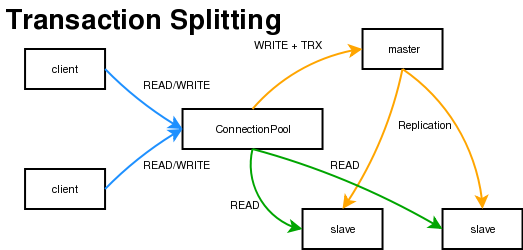
\includegraphics[keepaspectratio,width=0.5\paperwidth]{Pictures/Network/EbayRWSplitting.png}
	\caption{Ebay的读写分离}
	\label{fig:VirtualServer}
	\end{center}
\end{figure}

\begin{figure}[ht]
	\begin{center}
		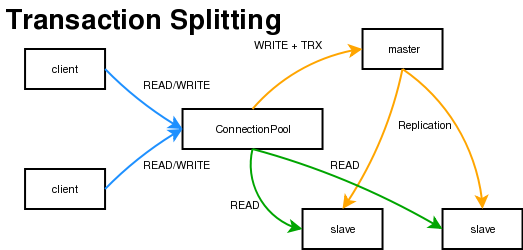
\includegraphics[keepaspectratio,width=0.5\paperwidth]{Pictures/Network/MySQLSplitting.png}
	\caption{MySQL的读写分离}
	\label{fig:VirtualServer}
	\end{center}
\end{figure}


Ebay使用Oracle的数据库,通过Quest SharePlex工具进行数据同步。

MySQL也有自己的同步数据技术, 通过日志在从数据库重复主数据库的操作达到异步复制数据目的。



\subsection{索引}

索引是对数据库表中一列或多列的值进行排序的一种结构,使用索引可快速访问数据库表中的特定信息。
建立索引的目的是加快对表中记录的\textbf{查找}或\textbf{排序}。为表设置索引要付出代价的:一是增加了数据库的存储空间,二是在插入和修改数据时要花费较多的时间(因为索引也要随之变动)。
数据库索引就是为了提高表的搜索效率而对某些字段中的值建立的目录 。

创建索引可以大大提高系统的性能。第一,通过创建唯一性索引,可以保证数据库表中每一行数据的唯一性。第二,可以大大加快数据的检索速度,这也是创建索引的最主要的原因。第三,可以加速表和表之间的连接,特别是在实现数据的参考完整性方面特别有意义。第四,在使用分组和排序子句进行数据检索时,同样可以显著减少查询中分组和排序的时间。第五,通过使用索引,可以在查询的过程中,使用优化隐藏器,提高系统的性能。

例如这样一个查询:select * from table1 where id=10000。如果没有索引,必须遍历整个表,直到ID等于10000的这一行被找到为止;有了索引之后(必须是在ID这一列上建立的索引),即可在索引中查找。由于索引是经过某种算法优化过的,因而查找次数要少的多的多。可见,索引是用来定位的。

索引分为\textbf{聚簇索引}和\textbf{非聚簇索引}两种,聚簇索引是按照数据存放的物理位置为顺序的,而非聚簇索引就不一样了;聚簇索引能提高多行检索的速度,而非聚簇索引对于单行的检索很快。

根据数据库的功能,可以在数据库设计器中创建三种索引:唯一索引、主键索引和聚集索引。


唯一索引是不允许其中任何两行具有相同索引值的索引。
当现有数据中存在重复的键值时,大多数数据库不允许将新创建的唯一索引与表一起保存。数据库还可能防止添加将在表中创建重复键值的新数据。例如,如果在employee表中职员的姓(lname)上创建了唯一索引,则任何两个员工都不能同姓。

在数据库关系图中为表定义主键将自动创建主键索引,主键索引是唯一索引的特定类型。该索引要求主键中的每个值都唯一。当在查询中使用主键索引时,它还允许对数据的快速访问。

在\textbf{聚集索引}中,表中行的物理顺序与键值的逻辑(索引)顺序相同。一个表只能包含一个聚集索引。
如果某索引不是聚集索引,则表中行的物理顺序与键值的逻辑顺序不匹配。与非聚集索引相比,聚集索引通常提供更快的数据访问速度。

\textbf{应该在这些列上创建索引}

\begin{itemize}
    \item 
在经常需要搜索的列上,可以加快搜索的速度
    \item 
在作为主键的列上,强制该列的唯一性和组织表中数据的排列结构
    \item 
在经常用在连接的列上,这些列主要是一些外键,可以加快连接的速度;
    \item 
在经常需要根据范围进行搜索的列上创建索引,因为索引已经排序,其指定的范围是连续的;
    \item 
在经常需要排序的列上创建索引,因为索引已经排序,这样查询可以利用索引的排序,加快排序查询时间;
    \item 
在经常使用在WHERE子句中的列上面创建索引,加快条件的判断速度
\end{itemize}

\textbf{不应该在这些列上创建索引}

\begin{itemize}
    \item 
第一,对于那些在查询中很少使用或者参考的列不应该创建索引。这是因为,既然这些列很少使用到,因此有索引或者无索引,并不能提高查询速度。相反,由于增加了索引,反而降低了系统的维护速度和增大了空间需求。
    \item 
第二,对于那些只有很少数据值的列也不应该增加索引。这是因为,由于这些列的取值很少,例如人事表的性别列,在查询的结果中,结果集的数据行占了表中数据行的很大比例,即需要在表中搜索的数据行的比例很大。增加索引,并不能明显加快检索速度。
    \item 
第三,对于那些定义为text, image和bit数据类型的列不应该增加索引。这是因为,这些列的数据量要么相当大,要么取值很少,不利于使用索引。
    \item 
第四,当修改性能远远大于检索性能时,不应该创建索引。这是因为,修改性能和检索性能是互相矛盾的。当增加索引时,会提高检索性能,但是会降低修改性能。当减少索引时,会提高修改性能,降低检索性能。因此,当修改操作远远多于检索操作时,不应该创建索引。
\end{itemize}

\clearpage














%!Mode:: "TeX:UTF-8"
\section{关系数据库}

数据模型的三要素是\textbf{数据结构、数据操作和完整性约束}。根据数据结构的不同,常见的数据模型包括\textbf{层次模型,网状模型和关系模型}。

\textbf{实体完整性}要求每一个表中的主键字段都不能为空或者重复的值。
\textbf{域完整性}限制了某些属性中出现的值,把属性限制在一个有限的集合中。例如,如果属性类型是整数,那么它就不能是101.5或任何非整数。
\textbf{引用完整性}表示任何引用表中的外键都必须总引用被引用表中的一个有效行。引用完整性确保两表间的关系在更新和删除期间保持同步。
如果要删除被引用的对象,那么也要删除引用它的所有对象,或者把引用值设置为空(如果允许的话)。
\textbf{用户定义完整性}(user defined integrity)则是根据应用环境的要求和实际的需要,对某一具体应用所涉及的数据提出约束性条件。
这一约束机制一般不应由应用程序提供,而应有由关系模型提供定义并检验。

设FK是基本关系R的一个或一组属性,但不一定是关系R的主关键字。如果FK与基本关系S的主关键字相对应,则称FK是基本关系R的外关键字,并称基本关系R为引用关系,基本关系S为被引用关系。

\subsection{关系数据库的设计范式}
\textbf{第一范式(1NF)}是指数据库表的每一列都是不可分割的基本数据项,同一列中不能有多个值,即实体中的某个属性不能有多个值或者不能有重复的属性。

\textbf{第二范式}要求数据表里的所有数据都要和该数据表的主键有完全依赖关系;如果有哪些数据只和主键的一部份有关的话,就得把它们独立出来变成另一个数据表。如果一个数据表的主键只有单一一个字段的话,它就一定符合第二范式。所谓\textbf{完全依赖}是指不能存在仅依赖主关键字一部分的属性。

\textbf{第三范式}需要确保数据表中的每一列数据都和候选码直接相关,而不能间接相关。
若$R \in 3NF$,则$R$的每一个非主属性既不部分函数依赖于候选码也不传递函数依赖于候选码。

\textbf{BC范式(BCNF,3.5NF)}
是在第三范式的基础上加上更严格约束,每个BCNF关系是第三范式的子集,有从属关系。它的定义是:
如果对于关系模式$R \in 1NF$中存在的任意一个\textbf{非平凡函数依赖}(非平凡指A不说X子集)$X \to A$,都满足X是R的一个候选键,那么关系模式$R \in BCNF$。

函数依赖和多值依赖是两种最重要的数据依赖。如果只考虑函数依赖,则修正第三范式后的BCNF的关系模式规范化程度已经是最高的了。
\textbf{第四范式}涵义:$R \in 1NF$,如果对于R的每个非平凡多值依赖$X \to \to Y$,X都含有候选码,则$R \in 4NF$。
设R(U)是属性集U上的一个关系模式。X,Y,Z是U的子集,并且Z=U-X-Y。关系模式R(U)中\textbf{多值依赖}$X \to \to Y$成立,当且仅当对R(U)的任一关系r,给定的一对(x,z)值有一组Y的值,这组值仅仅决定于x值而与z值无关。若$X \to \to Y$,而Z为空集,则称$X \to \to Y$为平凡的多值依赖;若Z不为空,则称其为非平凡的多值依赖。


\subsection{流行的关系数据库}

\textbf{MySQL} 5作为当今最流行的开放源码数据库之一,MySQL数据库为用户提供了一个相对简单的解决方案,适用于广泛的应用程序部署,能够降低用户的TCO。
MySQL是一个多线程、结构化查询语言(SQL)数据库服务器。MySQL的执行性能高, 运行速度快,容易使用。

\textbf{PostgreSQL}是一个功能齐全、开放源码的对象一关系性数据库管理系统 (ORDBMS)。目前,PostgreSQL的稳定版本为8.4版,具有丰富的特性和商业级数据库管理系统的特质。这是一次向高质量大型数据库管理系统方向的飞跃。
PostgreSQL是很富特色的开源数据库管理系统,其特性覆盖SQL-2/SQL-92和SQL-3/SQL-99。


商用数据库包括IBM DB2,Oracle,Informix,Sybase,SQL Server。

\subsection{关系代数}

投影(projection)操作用来从关系R中生成一个新的关系,包含R的部分列,记作$\pi_{A_1,A_2,\dots,A_n}(R)$。

选择(selection)操作作用到R上,产生的新关系的元组必须满足涉及某属性的条件C,记作$\sigma_C(R)$。

\textbf{内连接}包括\textbf{相等连接},\textbf{自然连接},\textbf{$\theta$连接}和\textbf{交叉连接}等。

\textbf{交叉连接}(cross join),又称\textbf{笛卡尔连接}(cartesian join)或叉乘(Product),它是所有类型的内连接的基础。把表视为行记录的集合,交叉连接即返回这两个集合的笛卡尔积。这其实等价于内连接的链接条件为"永真",或连接条件不存在.如果 A 和 B 是两个集合,它们的交叉连接就记为: A × B.用于交叉连接的 SQL 代码在 FROM 列出表名,但并不包含任何过滤的连接谓词.
显式的交叉连接实例:

\begin{verbatim}
SELECT *
FROM   employee CROSS JOIN department
\end{verbatim}

隐式的交叉连接实例:

\begin{verbatim}
SELECT *
FROM   employee,department;
\end{verbatim}


\textbf{$\theta$连接}用于筛选出符合一定条件的元组。满足条件C的关系R和S的$\theta$连接记作$R \Join _{C} S$。

\textbf{相等连接} (equi-join,或 equijoin),是比较连接({$\theta$连接})的一种特例,它的连接谓词只用了相等比较。使用其他比较操作符(如 <)的不是相等连接。
\begin{verbatim}
SELECT *
FROM   employee 
INNER JOIN department 
ON employee.DepartmentID = department.DepartmentID
\end{verbatim}

\begin{verbatim}
SELECT *  
FROM   employee,department 
WHERE  employee.DepartmentID = department.DepartmentID
\end{verbatim}

 \textbf{自然连接}比相等连接的进一步特例化。两表做自然连接时,两表中的所有名称相同的列都将被比较,这是隐式的。自然连接得到的结果表中,两表中名称相同的列只出现一次。R与S的自然连接表示为$R \Join S$。

\begin{verbatim}
SELECT *
FROM   employee NATURAL JOIN department
\end{verbatim}

\textbf{外连接}并不要求连接的两表的每一条记录在对方表中都一条匹配的记录. 连接表保留所有记录 -- 甚至这条记录没有匹配的记录也要保留. 外连接可依据连接表保留左表, 右表或全部表的行而进一步分为左外连接, 右外连接和全连接.在标准的 SQL 语言中, 外连接没有隐式的连接符号.

\textbf{左外连接}(left outer join), 亦简称为左连接(left join), 若 A 和 B 两表进行左外连接, 那么结果表中将包含"左表"(即表 A)的所有记录, 即使那些记录在"右表" B 没有符合连接条件的匹配. 这意味着即使 ON 语句在 B 中的匹配项是0条, 连接操作还是会返回一条记录, 只不过这条记录的中来自于 B 的每一列的值都为 NULL. 这意味着左外连接会返回左表的所有记录和右表中匹配记录的组合(如果右表中无匹配记录, 来自于右表的所有列的值设为 NULL). 如果左表的一行在右表中存在多个匹配行, 那么左表的行会复制和右表匹配行一样的数量, 并进行组合生成连接结果.
\textbf{全连接}是左右外连接的并集. 连接表包含被连接的表的所有记录, 如果缺少匹配的记录, 即以 NULL 填充.一些数据库系统(如 MySQL)并不直接支持全连接, 但它们可以通过左右外连接的并集(union)来模拟实现.

自连接就是和自身连接.

\begin{verbatim}
SELECT F.EmployeeID, F.LastName, S.EmployeeID, S.LastName, F.Country
FROM Employee F, Employee S
WHERE F.Country = S.Country
AND F.EmployeeID < S.EmployeeID
ORDER BY F.EmployeeID, S.EmployeeID
-- 雇员表 Employee
\end{verbatim}



















%!Mode:: "TeX:UTF-8"
\section{MySQL}


\subsection{Deploying MySQL}

Starting MySQL in Mac OS X:
\begin{lstlisting}
mysql.server start
\end{lstlisting}
If that fails, just type \verb|mysqld|.

To Create a database in MySQL,
\begin{lstlisting}
create database samp_db character set gbk;
CREATE DATABASE IF NOT EXISTS mdss DEFAULT CHARSET utf8 COLLATE utf8_general_ci;
\end{lstlisting}


To create a table, the official site of MySQL gives an example:
\begin{lstlisting}
 CREATE TABLE pet (name VARCHAR(20), owner VARCHAR(20), species VARCHAR(20), sex CHAR(1), birth DATE, death DATE);
\end{lstlisting}

Read meta data:
\begin{lstlisting}
desc haah;
describe haah;
show columns from haah;
SHOW CREATE TABLE tablename;
show full columns from haah;
\end{lstlisting}

Schema can be specified when login,
\begin{lstlisting}
mysql -D dbname -h hostname -u username -p
\end{lstlisting}

SQL statements or a script can also be specified during the login command,
\begin{lstlisting}
mysql -D samp_db -u root  < h.sql
mysql -D samp_db -u root  -e 'select * from haah;'
\end{lstlisting}


\subsection{Configuration}

Check timeout settings,
\begin{verbatim}
show variables where variable_name like '%timeout';
\end{verbatim}


You change default value in MySQL configuration file

\begin{verbatim}
[mysqld]
connect_timeout=100
\end{verbatim}

Or set this in statements like
\begin{verbatim}
con.query('SET GLOBAL connect_timeout=28800')
con.query('SET GLOBAL wait_timeout=28800')
con.query('SET GLOBAL interactive_timeout=28800')
\end{verbatim}

\subsection{security management}

If you have never set a root password for MySQL, the server does not require a password at all for connecting as root. To set up a root password for the first time, use the mysqladmin command at the shell prompt as follows:

\begin{verbatim}
mysqladmin -u root password NEWPASS 
\end{verbatim}

If you want to change (or update) a root password to the new password 'newpass', then you need to use the following command:

\begin{verbatim}
mysqladmin -u root -p OLDPASS NEWPASS 
\end{verbatim}

\subsection{MySQL with Python}

Installation on Windows:
\begin{verbatim}
install using wheel
pip install wheel
download from http://www.lfd.uci.edu/~gohlke/pythonlibs/#mysql-python
pip install mysqlclient-1.3.8-cp36-cp36m-win_amd64.whl
\end{verbatim}


\subsection{Data Export and Import with CSV files}

\begin{verbatim}

mysql -uroot -p123456 -hmdss18 -Dmdss -e "SELECT * FROM i_ddos_current_events
INTO OUTFILE '/tmp/i_ddos_current_events.csv'
FIELDS TERMINATED BY ','
ENCLOSED BY '\"'
LINES TERMINATED BY '\n';"

scp root@mdss18:/tmp/*_ddos_*.csv root@mdss27:/tmp

mysql -uroot -p123456 -hmdss27 -Dmdss -e "
TRUNCATE i_ddos_current_events;
LOAD DATA INFILE '/tmp/i_ddos_current_events.csv' REPLACE
INTO TABLE i_ddos_current_events
FIELDS TERMINATED BY ','
ENCLOSED BY '\"'
LINES TERMINATED BY '\n';

\end{verbatim}


\subsection{Data Migration via SQL Scripts}

\begin{verbatim}
mysqldump -uroot -p123456 -hmdss18 mdss i_ddos_flood_events --where 'id in
(select id from i_ddos_current_events)'
 --lock-tables=false --no-create-info --insert-ignore 
 > /tmp/i_ddos_flood_events.sql
 
 mysql -uroot -p123456 -hmdss27 -Dmdss --force < /tmp/i_ddos_flood_events.sql
\end{verbatim}

\subsection{MySQL Ping}
\begin{verbatim}
/* ping */ select 1
\end{verbatim}




%!Mode:: "TeX:UTF-8"
\section{NoSQL}


NoSQL有时也称作Not Only SQL的缩写,是对不同于传统的关联式数据库的数据库管理系统的统称。
两者存在许多显著的不同点,其中最重要的是NoSQL不使用SQL作为查询语言。
其数据存储可以不需要固定的表格模式,也经常会避免使用SQL的JOIN操作,一般有水平可扩展性的特征。
NoSQL的实现具有二个特征:使用硬盘,或者把随机存储器作存储载体。
少数NoSQL系统部署了分布式结构,通常使用分散式杂凑表(DHT)将数据以冗余方式保存在多台服务器上。依此,扩充系统时候添加服务器更容易,并且扩大了对服务器失效的承受能程度。


\subsection{BigTable}
BigTable是Google设计的分布式数据存储系统,用来处理海量的数据的一种非关系型的数据库。

BigTable是非关系的数据库,是一个稀疏的、分布式的、持久化存储的多维度排序Map。Bigtable的设计目的是可靠的处理PB级别的数据,并且能够部署到上千台机器上。Bigtable已经实现了下面的几个目标:适用性广泛、可扩展、高性能和高可用性。Bigtable已经在超过60个Google的产品和项目上得到了应用,包括 Google Analytics、GoogleFinance、Orkut、Personalized Search、Writely和GoogleEarth。这些产品对Bigtable提出了迥异的需求,有的需要高吞吐量的批处理,有的则需要及时响应,快速返回数据给最终用户。它们使用的Bigtable集群的配置也有很大的差异,有的集群只有几台服务器,而有的则需要上千台服务器、存储几百TB的数据。

在很多方面,Bigtable和数据库很类似:它使用了很多数据库的实现策略。并行数据库和内存数据库已经具备可扩展性和高性能,但是Bigtable提供了一个和这些系统完全不同的接口。Bigtable不支持完整的关系数据模型;与之相反,Bigtable为客户提供了简单的数据模型,利用这个模型,客户可以动态控制数据的分布和格式(alex注:也就是对BigTable而言,数据是没有格式的,用数据库领域的术语说,就是数据没有Schema,用户自己去定义Schema),用户也可以自己推测(alex注:reasonabout)底层存储数据的位置相关性(alex注:位置相关性可以这样理解,比如树状结构,具有相同前缀的数据的存放位置接近。在读取的时候,可以把这些数据一次读取出来)。数据的下标是行和列的名字,名字可以是任意的字符串。Bigtable将存储的数据都视为字符串,但是Bigtable本身不去解析这些字符串,客户程序通常会在把各种结构化或者半结构化的数据串行化到这些字符串里。通过仔细选择数据的模式,客户可以控制数据的位置相关性。最后,可以通过BigTable的模式参数来控制数据是存放在内存中、还是硬盘上。

\subsection{HBase}

HBase是一个开源的非关系型分布式数据库(NoSQL),它参考了谷歌的BigTable建模,实现的编程语言为Java。
它是Apache软件基金会Hadoop项目的一部分,运行于HDFS文件系统之上,为Hadoop提供类似于BigTable规模的服务。HBase在列上实现了BigTable论文提到的压缩算法、内存操作和布隆过滤器。

HBase – Hadoop Database,是一个高可靠性、高性能、面向列、可伸缩的分布式存储系统,利用HBase技术可在廉价PC Server上搭建起大规模结构化存储集群。
HBase是Google Bigtable的开源实现,类似Google Bigtable利用GFS作为其文件存储系统,HBase利用Hadoop HDFS作为其文件存储系统;Google运行MapReduce来处理Bigtable中的海量数据,HBase同样利用Hadoop MapReduce来处理HBase中的海量数据;Google Bigtable利用 Chubby作为协同服务,HBase利用Zookeeper作为对应。
  
  
\subsection{mongodb}

MongoDB是一个高性能,开源,无模式的文档型数据库,是当前NoSql数据库中比较热门的一种。它在许多场景下可用于替代传统的关系型数据库或键/值存储方式。Mongo使用C++开发。

Mongo DB很好的实现了面向对象的思想(OO思想),在Mongo DB中 每一条记录都是一个Document对象。Mongo DB最大的优势在于所有的数据持久操作都无需开发人员手动编写SQL语句,直接调用方法就可以轻松的实现CRUD操作。

NoSQL数据库与传统的关系型数据库相比,它具有操作简单、完全免费、源码公开、随时下载等特点,并可以用于各种商业目的。
这使NoSQL产品广泛应用于各种大型门户网站和专业网站,大大降低了运营成本。
2010年,随着互联网Web2.0网站的兴起,NoSQL在国内掀起一阵热潮,其中风头最劲的莫过于MongoDB了。
越来越多的业界公司已经将MongoDB投入实际的生产环境,很多创业团队也将MongoDB作为自己的首选数据库,创造出非常之多的移动互联网应用。

MongoDB的文档模型自由灵活,可以让你在开发过程中畅顺无比。对于大数据量、高并发、弱事务的互联网应用,MongoDB可以应对自如。MongoDB内置的水平扩展机制提供了从百万到十亿级别的数据量处理能力,完全可以满足Web2.0和移动互联网的数据存储需求,其开箱即用的特性也大大降低了中小型网站的运维成本。

适用场合:
\begin{itemize}
\item 网站数据:Mongo非常适合实时的插入,更新与查询,并具备网站实时数据存储所需的复制及高度伸缩性。
\item 缓存:由于性能很高,Mongo也适合作为信息基础设施的缓存层。在系统重启之后,由Mongo搭建的持久化缓存层可以避免下层的数据源 过载。
\item 大尺寸,低价值的数据:使用传统的关系型数据库存储一些数据时可能会比较昂贵,在此之前,很多时候程序员往往会选择传统的文件进行存储。
\item 高伸缩性的场景:Mongo非常适合由数十或数百台服务器组成的数据库。Mongo的路线图中已经包含对MapReduce引擎的内置支持。
\item 用于对象及JSON数据的存储:Mongo的BSON数据格式非常适合文档化格式的存储及查询。
\end{itemize}


\subsection{Redis}
Redis是一个开源的使用ANSI C语言编写、支持网络、可基于内存亦可持久化的日志型、Key-Value数据库,并提供多种语言的API。
从2010年3月15日起,Redis的开发工作由VMware主持。

Redis是一个key-value存储系统。和Memcached类似,它支持存储的value类型相对更多,包括string(字符串)、list(链表)、set(集合)、zset(sorted set --有序集合)和hash(哈希类型)。这些数据类型都支持push/pop、add/remove及取交集并集和差集及更丰富的操作,而且这些操作都是原子性的。在此基础上,redis支持各种不同方式的排序。与memcached一样,为了保证效率,数据都是缓存在内存中。
区别的是redis会周期性的把更新的数据写入磁盘或者把修改操作写入追加的记录文件,并且在此基础上实现了master-slave(主从)同步。

Redis的外围由一个键、值映射的字典构成。与其他非关系型数据库主要不同在于:Redis中值的类型不仅限于字符串,还支持如下抽象数据类型:
\begin{itemize}
\item 字符串列表
\item 无序不重复的字符串集合
\item 有序不重复的字符串集合
\item 键、值都为字符串的哈希表
\end{itemize}
值的类型决定了值本身支持的操作。Redis支持不同无序、有序的列表,无序、有序的集合间的交集、并集等高级服务器端原子操作。

Redis通常将全部的数据存储在内存中。2.4版本后可配置为使用虚拟内存,一部分数据集存储在硬盘上,但这个特性废弃了。
目前通过两种方式实现持久化:
\begin{itemize}
\item 使用快照,一种半持久耐用模式。不时的将数据集以异步方式从内存以RDB格式写入硬盘。
\item 1.1版本开始使用更安全的AOF格式替代,一种只能追加的日志类型。将数据集修改操作记录起来。Redis能够在后台对只可追加的记录作修改来避免无限增长的日志。
\end{itemize}


Redis支持主从同步。数据可以从主服务器向任意数量的从服务器上同步,从服务器可以是关联其他从服务器的主服务器。这使得Redis可执行单层树复制。从盘可以有意无意的对数据进行写操作。由于完全实现了发布/订阅机制,使得从数据库在任何地方同步树时,可订阅一个频道并接收主服务器完整的消息发布记录。同步对读取操作的可扩展性和数据冗余很有帮助。


\subsection{Casssandra}
Cassandra最初由Facebook开发,后来成了Apache开源项目,它是一个网络社交云计算方面理想的数据库。它集成了其他的流行工具如Solr,现在已经成为一个完全成熟的大型数据存储工具。Cassandra是一个混合型的非关系的数据库,类似于Google的BigTable。其主要功能比Dynomite(分布式的Key-Value存储系统)更丰富,但支持度却不如文档存储MongoDB。Cassandra的主要特点就是它不是一个数据库,而是由一堆数据库节点共同构成的一个分布式网络服务,对Cassandra的一个写操作,会被复制到其他节点上去,而对Cassandra的读操作,也会被路由到某个节点上面去读取。在最近的一次测试中,Netflix建立了一个288个节点的集群。

\subsection{DynamoDB}
DynamoDB是亚马逊的key-value模式的存储平台,可用性和扩展性都很好,性能也不错:读写访问中99.9\%的响应时间都在300ms内。DynamoDB的NoSQL解决方案,也是使用键/值对存储的模式,平且通过服务器把所有的数据存储在SSD上的三个不同的区域。如果有更高的传输需求,DynamoDB也可以在后台添加更多的服务器。

\subsection{CouchDB}
CouchDB是用Erlang开发的面向文档的数据库系统,不过它不是一个传统的关系数据库,而是面向文档的数据库,其数据存储方式有点类似lucene的index文件格式,CouchDB最大的意义在于它是一个面向web应用的新一代存储系统。作为一个分布式的数据库,CouchDB可以把存储系统分布到n台物理的节点上面,并且很好的协调和同步节点之间的数据读写一致性。CouchDB支持REST API,可以让用户使用JavaScript来操作CouchDB数据库,也可以用JavaScript编写查询语句,可以想像一下,用AJAX技术结合CouchDB开发出来的CMS系统会是多么的简单和方便。


\subsection{Lucene/Solr}
Lucene是Apache软件基金会4 jakarta项目组的一个子项目,这是一个开放源代码的全文检索引擎工具包,就是说它不是一个完整的全文检索引擎,而是一个全文检索引擎的架构。不过大多数人并不认同Lucene是一个数据库,因为大多数人只是用它来检索大量的文本块,不过它的确采用了与其他NoSQL数据存储相似的模型。如果说查询并不是仅仅局限于精确的匹配,而是寻找出那些出现在块中的字或者字段的话,毫无疑问,Lucene/Solr是最好的查询方式。















%!Mode:: "TeX:UTF-8"
\section{Redis}

\subsection{Installation and Start}

To install on CentOS 6:
\begin{verbatim}
yum install epel-release
yum install redis
service redis start
\end{verbatim}

To start a redis client connecting to local server:
\begin{verbatim}
redis-cli
redis-cli -h 172.30.35.1 
\end{verbatim}

To allow remote access, modify redis.conf:
\begin{verbatim}
bind 0.0.0.0
\end{verbatim}

Before connecting to a remote database, we can first try to ping it:
\begin{verbatim}
redis-cli -h 172.30.35.1 ping
\end{verbatim}

Simple manipulation:
\begin{verbatim}
redis 127.0.0.1:6379> set age 22
OK
redis 127.0.0.1:6379> incr age
(integer) 23
redis 127.0.0.1:6379> get age
"24"
redis 127.0.0.1:6379> set name 'ka'
OK
redis 127.0.0.1:6379> get name
"ka"
\end{verbatim}

We can delete a key by using 
\begin{verbatim}
DEL keynname
\end{verbatim}


To list all keys matching a wildcard, type like this:
\begin{verbatim}
KEYS *
\end{verbatim}

\subsection{Programming Redis with Python}
Python API is provided with the \textbf{redis} package.

\begin{verbatim}
import redis
r = redis.Redis(host='localhost', port=6379, db=0)
x = r.get('age')
r.set('foo', 'bar')
y = r.get('foo')
\end{verbatim}










%!Mode:: "TeX:UTF-8"
\section{SQL}
SQL是介于关系代数和关系演算之间的结构化查询语言,已经成为关系数据库的标准语言。


SQL is a set-based, declarative query language, not an imperative language like C or BASIC. However, there are extensions to Standard SQL which add procedural programming language functionality, such as control-of-flow constructs. SQL/PSM (SQL/Persistent Stored Modules) is an ISO standard mainly defining an extension of SQL with a procedural language for use in stored procedures. However, the major SQL vendors have historically included their own proprietary procedural extensions. 

SQL包含3个部分:
\begin{itemize}
    \item 
“数据定义语言”(DDL : Data Definition Language)是SQL语言集中,负责数据结构定义与数据库对象定义的语言,由CREATE、ALTER与DROP三个语法所组成,最早是由 Codasyl (Conference on Data Systems Languages) 数据模型开始,现在被纳入 SQL 指令中作为其中一个子集。
    \item 
“数据操纵语言”(DML : Data Manipulation Language)负责对数据库对象运行数据访问工作的指令集,以INSERT、UPDATE、DELETE三种指令为核心,分别代表插入、更新与删除。Performing read-only queries of data is sometimes also considered a component of DML.有很多开发人员都把加上SQL的SELECT语句的四大指令以“CRUD”来称呼。SELECT \ldots INTO是非标准的持久化操作。
    \item 
“数据控制语言”(DCL : Data Control Language)是一种可对数据访问权进行控制的指令,它可以控制特定用户帐户对数据表、查看表、预存程序、用户自定义函数等数据库对象的控制权。由 GRANT 和 REVOKE 两个指令组成。
\end{itemize}

\begin{figure}[htpb]
    \begin{center}
        
\includegraphics[keepaspectratio,width=0.5\paperwidth]{Pictures/SqlANATOMY.png}
    \end{center}
    \caption{SQL language elements}
    \label{fig:SQL lan elem}
\end{figure}

某些数据库强制要求语句后有分号。

\subsection{真值逻辑}

空值(关键字NULL),关系数据库中对数据属性未知或缺失的一种标识。数据库表主键的取值不能为空值。在SQL的Where条件式去判断字段是否为Null时,where id = null 是无法正确执行的,必须写成 where id is null, 其否定条件是is not null。

三值逻辑:true, false, unknown。false AND unknown为false,true OR unknown为true。与null比较运算的结果是unknown.

expr1 IS NOT DISTINCT FROM expr2 表示二者的值相同或二者都为NULL。其否定为IS DISTINCT FROM。


\subsection{ANSI SQL数据类型}
\begin{itemize}
   \item 
 CHARACTER(n) or CHAR(n): fixed-width n-character string, padded with spaces as needed
   \item 
CHARACTER VARYING(n) or VARCHAR(n): variable-width string with a maximum size of n characters
   \item 
NATIONAL CHARACTER(n) or NCHAR(n): fixed width string supporting an international character set
   \item 
NATIONAL CHARACTER VARYING(n) or NVARCHAR(n): variable-width NCHAR string
   \item 
BIT(n): an array of n bits
   \item 
BIT VARYING(n): an array of up to n bits
   \item 
INTEGER and SMALLINT
   \item 
FLOAT, REAL and DOUBLE PRECISION
   \item 
NUMERIC(precision, scale) or DECIMAL(precision, scale),precision为有效数字位数,scale为小数位数
   \item 
DATE: for date values (e.g. 2011-05-03)
   \item 
TIME: for time values (e.g. 15:51:36). The granularity of the time value is usually a tick (100 nanoseconds).
   \item 
TIME WITH TIME ZONE or TIMETZ: the same as TIME, but including details about the time zone in question.
   \item 
TIMESTAMP: This is a DATE and a TIME put together in one variable (e.g. 2011-05-03 15:51:36).
   \item 
TIMESTAMP WITH TIME ZONE or TIMESTAMPTZ: the same as TIMESTAMP, but including details about the time zone in question.
\end{itemize}





\subsection{关键词}
关键词\textbf{DISTINCT}用于返回唯一不同的值。
\begin{verbatim}
SELECT DISTINCT 列名称 FROM 表名称
\end{verbatim}


\textbf{IN}操作符允许我们 WHERE子句中规定多个值。

\begin{verbatim}
SELECT column_name(s)
FROM table_name
WHERE column_name IN (value1,value2,...)
\end{verbatim}

操作符 \textbf{BETWEEN ... AND} 会选取介于两个值之间的数据范围。这些值可以是数值、文本或者日期。然而区间的开闭性因厂商而异。

\begin{verbatim}
SELECT column_name(s)
FROM table_name
WHERE column_name
BETWEEN value1 AND value2
\end{verbatim}

通过使用AS,可以为列名称和表名称指定别名(Alias)。

\begin{verbatim}
SELECT column_name(s)
FROM table_name
AS alias_name
\end{verbatim}

TOP 子句用于规定要返回的记录的数目。并非所有的数据库系统都支持 TOP 子句。
SQL Server 的语法: 
\begin{verbatim}
SELECT TOP number|percent column_name(s)
FROM table_name
\end{verbatim}

MySQL 语法:
\begin{verbatim}
SELECT column_name(s)
FROM table_name
LIMIT number
\end{verbatim}

Oracle 语法:
\begin{verbatim}
SELECT column_name(s)
FROM table_name
WHERE ROWNUM <= number
\end{verbatim}


\subsection{举例}

关系定义、删除与修改:
\begin{lstlisting}[language=SQL]
CREATE TABLE My_table(
 my_field1 INT,
 my_field2 VARCHAR(50),
 my_field3 DATE NOT NULL,
 PRIMARY KEY (my_field1, my_field2)
);

CREATE TABLE employees (
    id            INTEGER      PRIMARY KEY,
    first_name    VARCHAR(50)  NULL,
    last_name     VARCHAR(75)  NOT NULL,
    dateofbirth   DATE         NULL
);

CREATE TABLE MovieStar (
  name CHAR(30),
  address VARCHAR(255),
  gender CHAR(1),
  birthdate DATE
);

DROP TABLE My_table;

ALTER TABLE MovieStar ADD phone CHAR(3) NOT NULL;
ALTER TABLE MovieStar DROP birthdate;
\end{lstlisting}

索引创建与删除:
\begin{lstlisting}[language=SQL]
CREATE INDEX YearIndex ON Movie(year);
CREATE INDEX keyIndex ON Movie(title,year);
DROP INDEX YearIndex;
\end{lstlisting}

视图创建与删除:
\begin{lstlisting}[language=SQL]
CREATE VIEW ParamountMovie AS
  SELECT title, year
  FROM Movie
  WHERE studioName = 'Paramount';
  
CREATE VIEW MovieProd(movieTitle, prodName) AS
  SELECT title, year
  FROM Movie, MovieExe
  WHERE producerC# = cert#;
  
DROP VIEW ParamountMovie;
\end{lstlisting}

数据更新:
\begin{lstlisting}[language=SQL]
INSERT INTO My_table
 (field1, field2, field3)
 VALUES
 ('test', 'N', NULL);

UPDATE My_table
 SET field1 = 'updated value'
 WHERE field2 = 'N';

DELETE FROM My_table
 WHERE field2 = 'N';
 
TRUNCATE TABLE My_table;--清零
\end{lstlisting}

权限操作:
\begin{lstlisting}[language=SQL]
GRANT SELECT, UPDATE
 ON My_table
 TO some_user, another_user;
 
REVOKE SELECT, UPDATE
 ON My_table
 FROM some_user, another_user;
\end{lstlisting}

数据查询:
\begin{lstlisting}[language=SQL]
SELECT *
 FROM Book
 WHERE price > 100.00
 ORDER BY title;

 SELECT * FROM Persons
WHERE City LIKE 'N%'
--从"Persons" 表中选取居住在以 "N" 开始的城市里的人
--提示:"%" 可用于定义通配符(模式中缺少的字母)。


SELECT Book.title AS Title,
 COUNT(*) AS Authors
 FROM Book JOIN Book_author
 ON Book.isbn = Book_author.isbn
 GROUP BY Book.title;

SELECT * FROM Persons
WHERE LastName IN ('Adams','Carter')

SELECT * FROM Persons
WHERE LastName
BETWEEN 'Adams' AND 'Carter'

SELECT title,
 COUNT(*) AS Authors
 FROM Book NATURAL JOIN Book_author
 GROUP BY title;

SELECT isbn,
 title,
 price,
 price * 0.06 AS sales_tax
 FROM Book
 WHERE price > 100.00
 ORDER BY title;

SELECT isbn, title, price
 FROM Book
 WHERE price < (SELECT AVG(price) FROM Book)
 ORDER BY title;

SELECT Customer,SUM(OrderPrice) FROM Orders
GROUP BY Customer
-- 在 SQL 中增加 HAVING子句原因是,WHERE 关键字无法与合计函数一起使用。
HAVING SUM(OrderPrice)<2000

SELECT CASE WHEN i IS NULL THEN 'Null Result'  
-- This will be returned when i is NULL
            WHEN     i = 0 THEN 'Zero'         
-- This will be returned when i = 0
            WHEN     i = 1 THEN 'One'          
-- This will be returned when i = 1
            END
FROM t;

\end{lstlisting}


事务:
\begin{lstlisting}[language=SQL]
START TRANSACTION;
 UPDATE Account SET amount=amount-200 WHERE account_number=1234;
 UPDATE Account SET amount=amount+200 WHERE account_number=2345;
 
IF ERRORS=0 COMMIT;
IF ERRORS<>0 ROLLBACK;

CREATE TABLE tbl_1(id INT);
 INSERT INTO tbl_1(id) VALUES(1);
 INSERT INTO tbl_1(id) VALUES(2);
COMMIT;
 UPDATE tbl_1 SET id=200 WHERE id=1;
SAVEPOINT id_1upd;
 UPDATE tbl_1 SET id=1000 WHERE id=2;
ROLLBACK TO id_1upd;
 SELECT id FROM tbl_1;
\end{lstlisting}


\subsection{SQL 分页查询}

\begin{lstlisting}[language=SQL]
-- SQL SERVER
SELECT TOP 页大小 * FROM table1 WHERE id NOT IN ( SELECT TOP 页大小*(页数-1) id FROM table1 ORDER BY id ) ORDER BY id
--MYSQL
SELECT * FROM TT LIMIT startline, linecount
\end{lstlisting}
















%!Mode:: "TeX:UTF-8"
\section{sqlite3用法}
用法:
\begin{verbatim}
sqlite3 [options] [databasefile] [SQL]
\end{verbatim}

举例:
\begin{verbatim}
sqlite3 -line mydata.db 'select * from memos where priority > 20;'
sqlite3 bankinfo.db 'select * from BAcounts'
\end{verbatim}

\subsection{basic navigation}
\begin{verbatim}
.help
.schema ?TABLE?: Show the CREATE statements.
databases: List names and files of attached databases
.tables: Shows all tables
\end{verbatim}

\subsection{backup and restore}
\begin{verbatim}
.backup ?DB? FILE
.restore ?DB? FILE 
\end{verbatim}

\subsection{SQL脚本}
执行SQL脚本
\begin{verbatim}
.read filename
\end{verbatim}

输出SQL脚本
\begin{verbatim}
.output filename 
.dump
\end{verbatim}

\subsection{时间与日期}

\begin{verbatim}
select date('now')
\end{verbatim}

Python接口示例

\begin{lstlisting}[language=Python]
  def add_due_field(self):
        conn = sqlite3.connect(self.dbname)
        c = conn.cursor()
        c.execute('''DROP TABLE Fix2''')
        c.execute('''CREATE TABLE Fix2 
        		(start_date text, duration integer, 
        		end_date text, amount real, rate real, 
        		end_amount real, bank text)''')
        for record in self.items:
            start_date = datetime.strptime(
            		record[start_date_field], '%Y-%m-%d')
            start_date = start_date.date()
            duration_months = record[duration_field]
            principal = record[amount_field]
            rate = record[rate_field]
            bank = record[bank_field]
            end_date = TermDepositManager.__get_due_date__
            		(start_date, duration_months)
            due_value = TermDepositManager.__get_due_value__
            		(principal, duration_months, rate/100.0) 
            detail_record = (start_date, 
            		duration_months, end_date, principal, rate, due_value, bank)
            statement = "INSERT INTO Fix2 VALUES ('%s', %d, '%s', %f, %f, %.2f, '%s')" % detail_record; 
            c.execute(statement)

        conn.commit()
        conn.close()
\end{lstlisting}
















\end{document}
